%%%%%%%%%%%%%%%%%%%%%%%%%%%%%%%%%%%%%%%%%%%%%%%%%%%%%%%%%%
%% Task 3
%%%%%%%%%%%%%%%%%%%%%%%%%%%%%%%%%%%%%%%%%%%%%%%%%%%%%%%%%%

%%%%%%%%%%%%%%%%%%%%%%%%%%%%%%%%%%%%%%%%%%%%%%%%%%%%%%%%%%%%%%%
\subsubsection{e-Motions-based solution.}

\begin{figure}[htp]
  \centering
  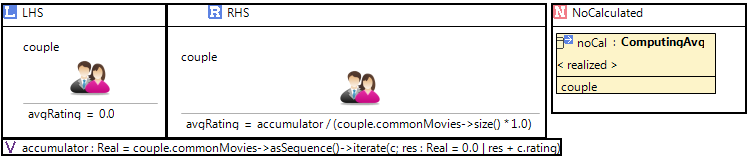
\includegraphics[width=\textwidth]{imgs/computingAvgRating}
  \caption{\code{computingAvgRating} rule.}\label{fig:computingAvgRating}
\end{figure}

\begin{table}
  \begin{center}
	\begin{tabular}{r r r}
	$N$ & Time (s) & \# Rewrites \\
	\hline
	2 & 0.0 & 4527 \\
	10 & 2.1 & 891432 \\
	\hline \\
	\end{tabular}
	\caption{e-Motions times for Task 23.}\label{table:emotionstask3}
	\end{center}
\end{table}

%%%%%%%%%%%%%%%%%%%%%%%%%%%%%%%%%%%%%%%%%%%%%%%%%%%%%%%%%%%%%%%
\subsubsection{Maude-based solution.}

\begin{lstlisting}[caption=Maude rule for Task 3 solution., label=lst:task3]
crl [avgRating] :
  { < M : Couple | commonMovies : MovieSet, avgRating : 0.0, Atts1 >
    couplesCalculated((Couples)) C 
  }
=>
  { < M : Couple | commonMovies : MovieSet, 
       avgRating : (sumAllRatings(MovieSet, C) / float(| MovieSet |)),
       Atts1 >
       couplesCalculated((M, Couples)) C
  }
if not(M in Couples) .
\end{lstlisting}

\begin{table}
  \begin{center}
	\begin{tabular}{r r r}
	$N$ & Time (s) & \# Rewrites \\
	\hline
	100 & 1.5 & 21800 \\
	200 & 6.3 & 43600 \\
	300 & 14.9 & 65400 \\
	400 & 29.7 & 87200 \\
	\hline \\
	\end{tabular}
	\caption{Maude times for Task 23.}\label{table:maudetask3}
	\end{center}
\end{table}